\documentclass[11pt,xcolor=svgnames]{beamer}
\usepackage{dsfont,natbib,setspace,changepage,multirow}
\mode<presentation>

% replaces beamer foot with simple page number
\setbeamertemplate{navigation symbols}{}
\setbeamerfont{frametitle}{series=\bfseries,size=\normalsize}
\setbeamercolor{frametitle}{fg=Black}

\setbeamertemplate{footline}{
   \raisebox{5pt}{\makebox[\paperwidth]{\hfill\makebox[20pt]{\color{gray}\scriptsize\insertframenumber}}}}

\usepackage{algorithm}
\usepackage{algorithmic}

% colors
\newcommand{\theme}{\color{Maroon}}
\newcommand{\bk}{\color{black}}
\newcommand{\rd}{\color{DarkRed}}
\newcommand{\fg}{\color{ForestGreen}}
\newcommand{\bl}{\color{blue}}
\newcommand{\gr}{\color{black!50}}
\newcommand{\sg}{\color{DarkSlateGray}}
\newcommand{\nv}{\color{Navy}}
\setbeamercolor{itemize item}{fg=gray}

% common math markups
\newcommand{\bs}[1]{\boldsymbol{#1}}
\newcommand{\mc}[1]{\mathcal{#1}}
\newcommand{\mr}[1]{\mathrm{#1}}
\newcommand{\bm}[1]{\mathbf{#1}}
\newcommand{\ds}[1]{\mathds{#1}}
\newcommand{\indep}{\perp\!\!\!\perp}
\def\plus{\texttt{+}}
\def\minus{\texttt{-}}

% spacing and style shorthand
\setstretch{1.1}

\begin{document}

\setcounter{page}{0}
{ \usebackgroundtemplate{
\includegraphics[height=\paperheight]{phoenix}}
\begin{frame}[plain]
\begin{center}


{\bf \Large Measuring Rhetoric}


\vskip 1cm
Matt Taddy,  Chicago Booth


\vskip .25cm
{\texttt{faculty.chicagobooth.edu/matt.taddy/research}}


\end{center}
\end{frame} }


\begin{frame}
{History: \theme Text as data}

Social science text-as-data from the 1960s: \\~~~author identification in the Federalist papers.
\begin{center}

\includegraphics[width=3.75in]{graphs/mostellerwallace}
\end{center}

\vskip -.5cm

\end{frame} 

\begin{frame}


M{\tt+}W count words in papers by Hamilton and Madison,
\begin{center}
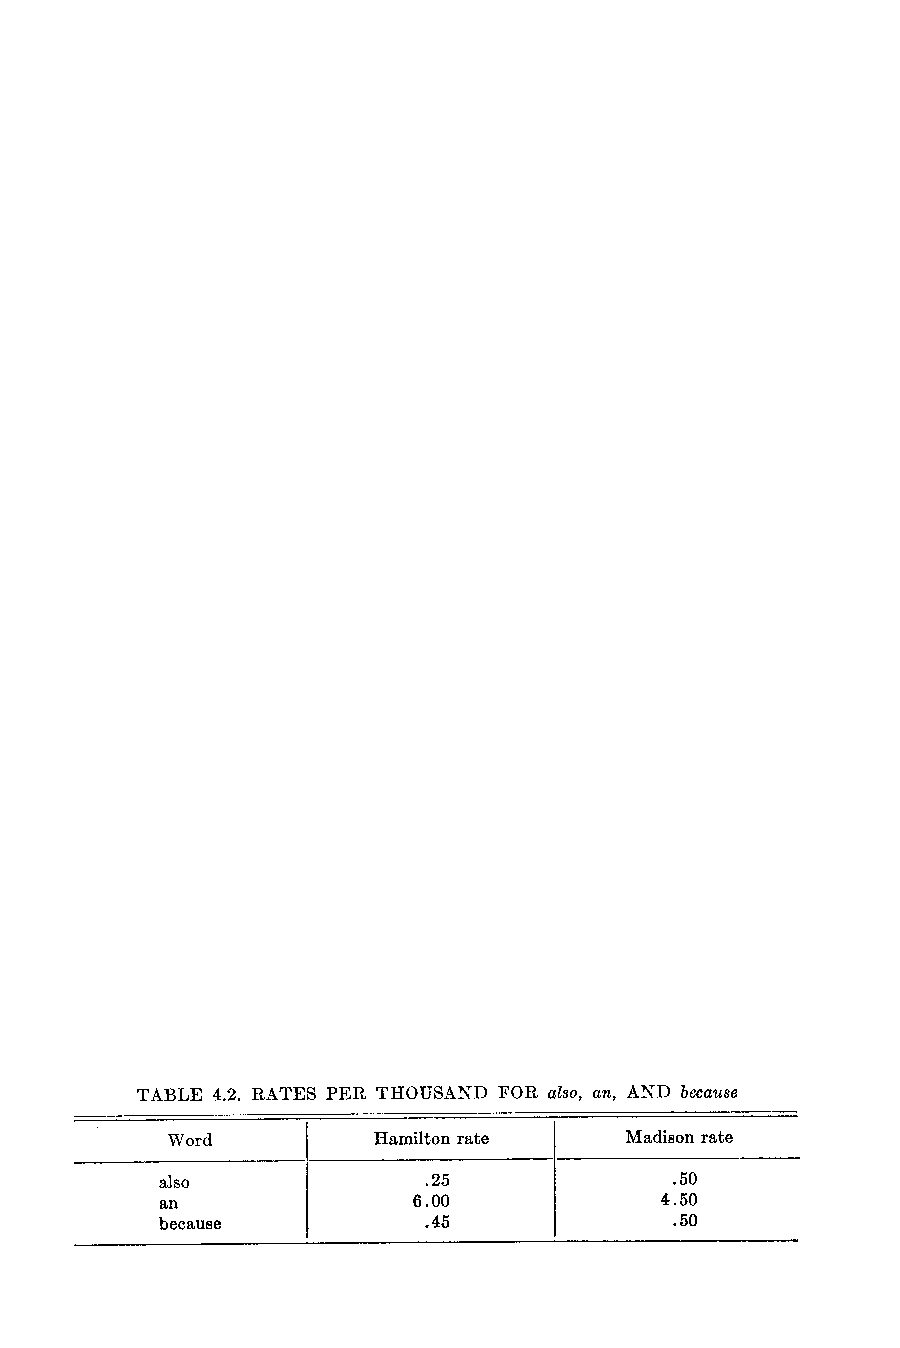
\includegraphics[width=4.25in]{graphs/mostellertab}
\end{center}


then fit models for counts$|$author {\gr (essentially what I use today!)},
and use Bayes rule to predict authors$|$counts on disputed work.

{\large \nv\[\mr{p}(\text{Hamilton}\mid \text{text}) \approx 
\frac{\mr{p}(\text{text} \mid \text{Hamilton})}
{\mr{p}(\text{text} \mid \text{Madison}) + \mr{p}(\text{text} \mid \text{Hamilton})}
\]}

\end{frame}


\begin{frame}{
The `{\theme bag of words}'}

\vskip .25cm
 A `word' is a self-contained meaningful token...

\begin{itemize}
\item Actual words: `all', `world', `stage', `:-)', `{\tt \#textdata}'.
\item n-grams: `merely players' (bi), `men and women' (tri)
\item complicated clauses: parts of speech, act-of-god.
\item user selections on a website, domain ids in browser history 
\end{itemize}

All we do is count them.

\vskip .5cm

{\nv The remains state of the art!}

\vskip .1cm
Treat tokens for each doc as an i.i.d. sample. 

\vskip .1cm
{\theme Document $i$ is summarized by counts $c_{ij}$ for tokens $j=1...d$.}

\vskip .1cm
Dumb but works: extra rules aren't worth their complexity.

\end{frame}

\begin{frame}
{Text as data \bk in Social Science}

\vskip .25cm
There's been an explosion of interest from social scientists.

 \vskip .25cm
Until very recently, one used pre-defined dictionaries.


\vskip .25cm
{Picking words: culturomics, Michel et al, Science 2011.}
\begin{center}
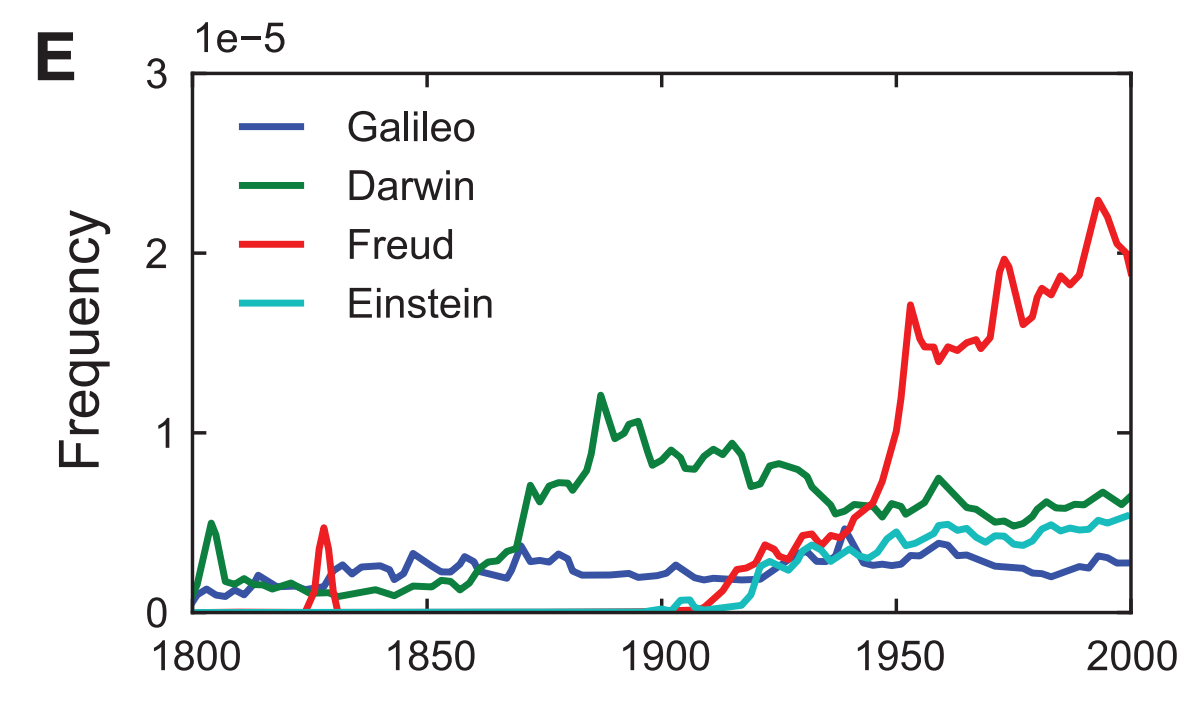
\includegraphics[width=2in]{graphs/culturomics}
\end{center}


Psychosocial dictionaries, such as Harvard GI in {\it Tetlock 2007, Giving Content to Investor Sentiment} and others: 
\begin{center}
{\color{DarkGreen} able, abundant, accept} vs 
{\color{DarkRed} abandon, abrupt, absurd}.
\end{center}

\end{frame}

\begin{frame}
{Topic Models}

\vskip .25cm
Techniques from stats and ML are beginning to filter through and researchers are estimating relationships {\it from the data}.

\vskip .25cm  
A large area of research has developed around {\it topic models} 
\[\nv
\bm{c}_i \sim \text{MN}( \omega_{i1} \bs{\theta}_1 + \ldots + \omega_{iK} \bs{\theta}_K, m_i)
\]
{a multinomial with probabilities $\sum_k \omega_{ik}\bs{\theta}_{k}$ and size $m_i= \sum_jc_{ij}$.}

\vskip .25cm
{\gr\hfill\it (Latent Dirichlet Allocation; Blei, Ng, Jordan 2003)~~~}

\vskip .5cm
This is a factor model for count data.


\end{frame}

\begin{frame}

Topics provide low-D structure, which the SS interprets.

{\gr Especially common in PoliSci; King, Grimmer, Quinn, ...}


\begin{center}
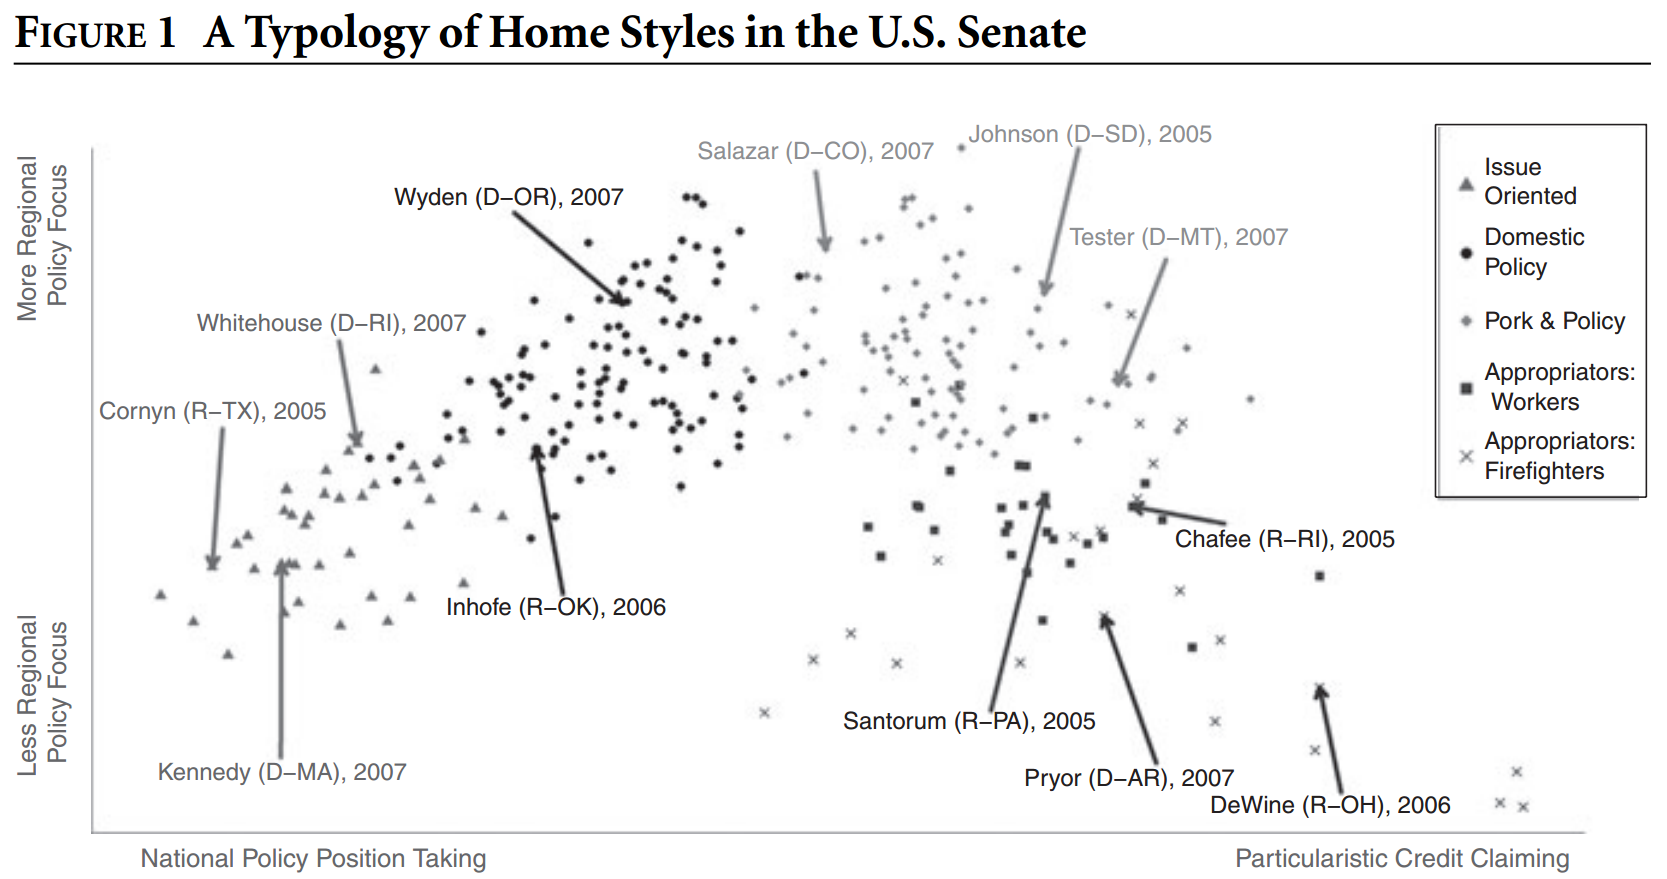
\includegraphics[width=3.75in]{graphs/grimmer}
\end{center}


{\it Grimmer 2013:}  fit latent topics in press releases \\(e.g., `Iraq', `Infastructure') then investigate who uses what topic.

\end{frame}

\begin{frame}
{Structured topic models}

The basic topic model finds {\it dominant sources of variation} in $\bm{C}$.

\vskip .1cm
In SocSci, this is often not what we're seeking (needle \texttt{+} haystack).

\vskip .5cm
There is a huge industry on extensions to topic models that push the topics to be relevant or interpretable for specific questions. \\\hfill{\gr supervised TM, dynamic TM, structural TM, IR TM ...~~~~~}

\vskip .5cm
These model weights ($\omega$) and topics ($\theta$) as functions of covariates.

\vskip .1cm
Lots of good and interesting work.



\end{frame}

\begin{frame}
{Multinomial Regression}

Instead of jumping straight to latent structure, perhaps we can answer our questions by regressing the text onto observables `$\bm{v}$'.


\vskip .5cm
Massive response {\nv logistic regressions}: 


\vskip .2cm ~~~~$\bm{c}_i \sim \mr{MN}(\bm{q}_i, m_i)~~\text{with}~~
q_{ij} = e^{\eta_{ij}}/\sum_l e^{\eta_{il}}$

\vskip .2cm ~~~~${\nv  \eta_{ij} = \alpha_j + \bm{v}_i'\bs{\varphi}_{j}}$ is a `log intensity'  {\gr $\approx \mathrm{E}\log(c_{ij}/m_i)$}

\vskip .5cm
This is a regression like any other.   

\vskip .2cm
We will be estimating {\it partial correlations}, can build {\it random effects} and {\it interactions} into $\bm{v}$, ...  all our familiar regression ideas apply.

\vskip .25cm
{\gr \it MN Inverse Regression \texttt{+} rejoinder, 2013.  Political Sentiment on Twitter, 2013.  Distributed MN Regression, 2015.}
\end{frame}

\begin{frame}
{Distributed Multinomial Regression}

{\gr A regression like any other, except the response is super HD. }

We approximate the MN likelihood with {\it independent} Poissons: 
{\large \nv \[
c_{ij} \sim \mr{Po}(~m_ie^{\eta_{ij}}~)
\]}
$\Rightarrow$ you can estimate each regression fully independently!

\vskip .5cm
This works because MN dependence is {\it only  induced by  totals}.

% \vskip -.35cm
% \[
% \mr{MN}\left(\bm{c}_i;~\bs{\pi}_{i}/\Pi_i,
% ~m_i\right) = \frac{\prod_j
% \mr{Po}\left(c_{ij};~\pi_{ij}\right)}
% {\mr{Po}\left(m_i;~\Pi_i\right)}~~\text{where}~~\Pi_i = \sum_j \pi_{ij}
% \]

\vskip .25cm
DMR is equivalent to MN logit in a variety of simple examples,\\ and is shown empirically to perform well in more complex settings.

\vskip .25cm
Everything in distribution: estimation, penalization, selection ...
\end{frame}

\begin{frame}

More precisely, start from the Poisson:
\[
c_{ij}\stackrel{ind}{\sim}\mathrm{Pois}\left(\exp\left[\mu_{i}+\eta_{ij}\right]\right)
\]
where $\mu_{i}$ is a `verbosity' nuisance parameter.


\vskip .1cm
This model leads to 
\[
\Pr\left(\mathbf{c}_{i}\mid m_{i}\right)=\frac{\prod_{j}\mathrm{Po}\left(c_{ij};\exp\left[\mu_{i}+\eta_{ij}\right]\right)}{\mathrm{Po}\left(m_{i};\sum_{l}\exp\left[\mu_{i}+\eta_{il}\right]\right)}=\mathrm{MN}(\mathbf{c}_{i};\mathbf{\,\, q}{}_{i},m_{i})
\]
Thus, given $m_i$, Poisson and MN imply the same  model.

\vskip .1cm
DMR fixes $\hat \mu_i = \log m_i$, so LHD factorizes to independent Poissons.


\vskip .5cm{\gr
More generally: for Big Data, consider using plug-in [marginal] estimates of parameters about which you have little uncertainty.  \\Focus computation on the bits that are hard to measure.}


\end{frame}

\begin{frame}
{Yelp Reviews}

We'll illustrate using {\theme publicly available} review data from Yelp.

\vskip .2cm
\begin{itemize}
\item $n=$ 215,879 reviews on 11,535 businesses by 43,873
users.
\item taken around Phoenix AZ on January 19, 2013.
\item $d=$ 13,938 words in more than 20 reviews.  
\end{itemize}

\vskip .2cm
The reviews are marked with review, business, and user attributes: number of stars, user and business star averages, business type (333 overlapping), and {\theme the number of funny/useful/cool votes.}

\end{frame}

\begin{frame}

Each {\it word-j} intensity regression equation has
\[
\eta_{ij} = \alpha_j + \bm{a}_i'\bs{\varphi}_j^a+ \bm{b}_i'\bs{\varphi}_j^b
\]
where we've resolved the meta-data attributes $\bm{V} = [~\bm{A} ~\bm{B}~]$\\ into variables of primary interest  and those viewed as controls
\begin{itemize}
\item[\bk \bf a:] star and vote counts; 11 dimensional.
\item[\bk \bf b:] 400 categories and 11,500 business random effects.
\end{itemize}


\vskip .5cm
Estimate parameters to minimize the penalized Poisson deviance
\[
\hat\alpha_j,\bs{\hat\varphi}_j = 
 \mathrm{argmin} \left\{l(\alpha_j,\bs{\varphi}_j) + n \lambda \left[\sum_k \omega^a_{jk} |\varphi^a_{jk} | + \frac{1}{\tau}\sum_k \omega^b_{jk} |\varphi^b_{jk} |\right]\right\}
\]
{\gr \it one-step estimator paths for concave regularization, 2015.}
\end{frame}

\begin{frame}

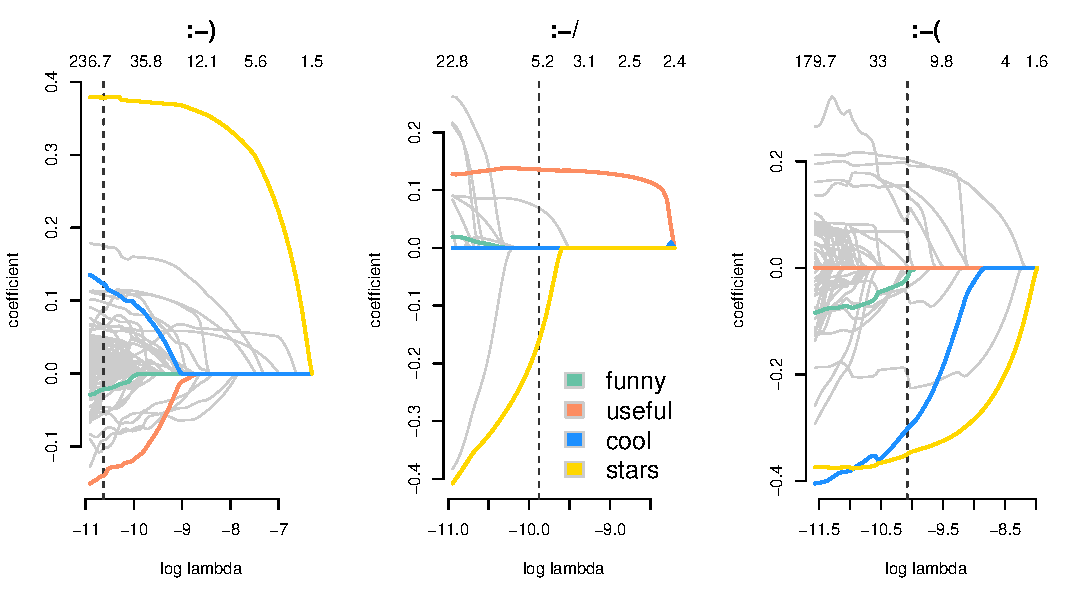
\includegraphics[width=\textwidth]{graphs/yelp_ir_paths}

\vskip .5cm
Poisson regression regularization paths under relative weight $\tau=2$.  

AICc selection is marked.

\end{frame}

\begin{frame}

{\bf\theme Resolving correlated effects}

\vskip .2cm
Bigger $\tau$ gives fewer but {\it cleaner} nonzero terms.

{\tiny\setstretch{1.25}\color{black!80}
\hspace{-.25cm}\begin{tabular}{cll|r}
& \scriptsize $\bs{\tau}$ & \scriptsize $|\bs{\hat\varphi}|_0$ 
& \scriptsize {\bf top ten words by loading}\\
\noalign{\smallskip}
\hline
 & \multicolumn{2}{l|}{marg}    & \tiny\it great love amaz favorite deliciou best awesome alway perfect excellent \\
\scriptsize +stars & 2 & 8440 & \tiny\it  unmatch salute :-)) prik laurie pheonix trove banoffee exquisite sublime \\
 & 20 & 3077 & \tiny\it  heaven perfection gem divine amaz die superb phenomenal fantastic deliciousnes \\
 & 200 & 508 & \tiny\it  gem heaven awesome wonderful amaz fantastic favorite love notch fabulou \\
\hline
&  \multicolumn{2}{l|}{marg}   & \tiny\it  not worst ask horrib minut rude said told would didn \\
\scriptsize -stars & 2 & 8440 & \tiny\it  rude livid disrespect disgrace inexcusab grosse incompet audacity unmelt acknowl \\
 & 20 & 3077 & \tiny\it  rude incompet unaccept unprofession inedib worst apolog disrespect insult acknowl \\
 & 200 & 508 & \tiny\it  worst horrib awful rude inedib terrib worse tasteles disgust waste \\
\hline
 & \multicolumn{2}{l|}{marg}   & \tiny\it  you that know like your yelp ... what don who \\
\scriptsize funny & 2 & 6508 & \tiny\it  dimsum rue reggae acne meathead roid bong crotch peni fart \\
 & 20 & 1785 & \tiny\it  bitch shit god dude boob idiot fuck hell drunk laugh \\
 & 200 & 120 & \tiny\it  bitch dear god hell face shit hipst dude man kidd \\
 \hline
 &  \multicolumn{2}{l|}{marginal}   & \tiny\it  that yelp you thi know biz-photo like all http :// \\
\scriptsize useful & 2 & 5230 & \tiny\it  fiancee rife dimsum maitre jpg poultry harissa bureau redirect breakdown \\
 & 20 & 884 & \tiny\it  biz-photo meow harissa www bookmark :-/ http :// (?), tip \\
 & 200 & 33 & \tiny\it  www http :// com factor already final immediate ask hope \\
\hline\end{tabular}}

\vskip .5cm
I think $\tau=20$ strikes a good balance here.

\vskip -.5cm
\end{frame}

\begin{frame}

{\bf \theme Sufficient Reduction}

\vskip .5cm
What is the funny/useful/cool content of a review?

\vskip .5cm
Coefficients $\bs{\Phi}$ are a linear map from text to attribute space.

\vskip .1cm
They provide a {\it sufficient reduction}. For example,
\[
\bm{a}_i \indep \bm{c}_i \mid
\bs{\Phi}^a \bm{c}_i, \bm{b}_i, m_i
\]
where $\bs{\Phi}^a$ are loadings relevant to our `primary interest' covariates.

\vskip .5cm
In words: the 11 dimensional $\theme \bm{z}_i = \bs{\Phi}^a \bm{c}_i$ contains all the information in the text that is {\it directly} relevant to $\bm{a}_i$, controlling for $\bm{b}_i$ and $m_i$.

\end{frame}

\begin{frame}

\footnotesize

{\bf Funniest and most useful 50-100 word review, as voted by Yelp users\\ {\gr (votes normalized by square root of review age).}}

\vskip .5cm{\it\color{black!70}\nv
I use to come down to Coolidge quite a bit and one of the cool things I use to do was come over here and visit the ruins.  A great piece of Arizona history!  Do you remember the Five C's?  Well, this is cotton country. The Park Rangers will tell you they don't really know how old the ruins are, but most guess at around 600 years plus.  But thanks to a forward thinking US Government, the ruins are now protected by a 70 foot high shelter.  Trust me, it comes in handy in July and August, the two months I seem to visit here most.  LOL.  I would also recommend a visit to the bookstore.  It stocks a variety of First Nation history, as well as info on the area.
  http://www.nps.gov/cagr/index.htm.  While you are in Coolidge, I would recommend the Gallopin' Goose for drinks or bar food, and Tag's for dinner.  Both are great!}

\end{frame}


\begin{frame}

\footnotesize

{\bf 50-100 word review with the most funny content, \\as measured by SR projection 
$\bs{z_{\texttt{funny}}} = \bs{\hat\phi}_{\texttt{funny}}'\bm{c}$.}

\vskip .25cm
{\it \nv Dear La Piazza al Forno: We need to talk. I don't quite know how to say this so I'm just going to come out with it. I've been seeing someone else. How long? About a year now. Am I in love? Yes. Was it you? It was. The day you decided to remove hoagies from your lunch menu, about a year ago, I'm sorry, but it really was you...and not me.  Hey... wait... put down that pizza peel... try to stay calm... please? [Olive oil container whizzing past head] Please! Stop throwing shit at me... everyone breaks up on social media these days... or haven't you heard?  Wow, what a Bitch!}

\vskip .75cm
{\bf most funny by $\bs{z_{\texttt{funny}}}/m$:} ~~~\textit{\nv Holy Mother of God}

\end{frame}

\begin{frame}

\footnotesize

{\bf 50-100 word review with the most useful content, \\as measured by SR projection 
$\bs{z_{\texttt{useful}}} = \bs{\hat\phi}_{\texttt{useful}}'\bm{c}$.}

\vskip .25cm
{\it \nv We found Sprouts shortly after moving to town.  There's a nice selection of Groceries \& Vitamins.  It's like a cheaper, smaller version of Whole Foods.
[biz-photo] [biz-photo] We shop here at least once a week.  I like their selection of Peppers....I like my spicy food! [biz-photo][biz-photo][biz-photo] Their freshly made Pizza isn't too bad either. [biz-photo] Overall, it's a nice shopping experience for all of us. Return Factor - 100\%}

\vskip .75cm
{\bf most useful by $\bs{z_{\texttt{useful}}}/m$:} ~~~\textit{\nv Ask for Nick!}

\end{frame}

\begin{frame}

The SR projections are based on {\it partial correlations}.  

\vskip .25cm
E.g., compare the correlation matrices
\begin{center}\vskip -.5cm
~~~~~~\begin{tabular}{r|ccccr|cccc}
 \multicolumn{4}{l}{\it attributes ($\bm{v}$)} & & 
 \multicolumn{4}{l}{\it \hskip .3cm text projections ($\bm{z}$)} \\ 
 %\multicolumn{10}{c}{}\\
\multicolumn{1}{c}{}& f & u &c & $\star$ &  \multicolumn{1}{c}{}&f & u &c & $\star$\\
\cline{2-5}\cline{7-10}
funny &  1 &  0.7 &  0.8 &   0 & \hskip .3cm funny &  1 &  -0.1 &  -0.7 &  -0.4\\
useful &  0.7 &  1 &  0.9 &   0 & \hskip .3cm useful &  -0.1 &  1 &  0.1 &  -0.2\\
cool &  0.8 &  0.9 &  1 &   0 & \hskip .3cm cool &  -0.7 &  0.1 &  1 &  0.5\\
stars &   0 &   0 &   0 &  1 & \hskip .3cm stars &  -0.4 &  -0.2 &  0.5 &  1\\
\end{tabular}
\end{center}

\vskip .5cm
SR projections make great inputs to prediction algorithms: {\theme MNIR}.

\end{frame}

\begin{frame}

{\bf Measuring Segregation in High Dimensions}

\vskip .05cm ~~~~{\it ~~~~with Matt Gentzkow and Jesse Shapiro}

\vskip .5cm
There's a big lit on measuring change in polarization/segregation.

\vskip .5cm
For example:
\begin{itemize} 
\item The $d$-vector  $\mathbf{c}_{tr} = [c_{tr1} \ldots c_{trd}]$ counts the number of members of race $r$ in each neighborhood
$j$ at time $t$.\\
{\color{black!50}
Or, compare across cities/countries/school districts/etc.}
\item 
Segregation measure maps counts $\left\{ \mathbf{c}_{tr}\right\} _{r=1}^{R}$
into scalar $s_{t}$
\item Use $s_1 \dots s_T$ to answer questions like
\item[]~~~~{\theme ``Has this city become more segregated over
time?''}
\end{itemize}

\vskip .5cm
Today's talk is about how to build $s_t$  when $d$ is really big.

\end{frame}


\begin{frame}

Current indices are derived from sets of stated desirable properties.


\vskip .5cm
Example: Atkinson index (Frankel and Volij 2010)
\[
s_{t} = 1 - \sum_{j} \sqrt{\frac{c_{t0j}}{m_{t0}}~
\frac{c_{t1j}}{m_{t1}}}
\]
for two groups (e.g., races) $r=0$ and $r=1$, where $m_{tr} = \sum_j c_{trj}$.

\vskip .5cm
This builds on an earlier literature that provides isolation, dissimilarity, mutual information, gini, and other indices.

\end{frame}


\begin{frame}

Are we after properties of the sample or of the DGP?

\vskip .2cm
That is, if the data are consistent with race-blind assignment do we
want to say that segregation is low?

\vskip .2cm
{\color{black!50} e.g., Cortese et al. (1976), Carrington and Troske (1997) both do.}

\vskip .5cm
Think of Atkinson as 
\[
\hat s_{t} = 1 - \sum_{j} \sqrt{\hat p_{t0j}~
\hat p_{t1j}}
\]
where $\mathbf{p}_{trj}$ is the true probability that a member of $r$ lives in $j$ at $t$. 


\vskip .5cm
This distinction is unimportant if $\hat s_t \approx s_t$.

\vskip .2cm
It is so for residential segregation because  zipcodes are large.

\vskip .2cm
But estimation bias becomes very important as units get smaller...

\end{frame}

\begin{frame}{Number of Districts Small}

1 million students

\begin{center}\vskip -1cm
\includegraphics[width=0.45\textwidth]{/home/taddy/project/politext/graphs/montecarlo/zipf_shorttail}
\end{center}
\vskip -2cm
\hfill 100 districts.

\end{frame}

\begin{frame}{Number of Districts Medium}

1 million students

\begin{center}\vskip -1cm
\includegraphics[width=0.45\textwidth]{/home/taddy/project/politext/graphs/montecarlo/zipf_mediumtail}
\end{center}
\vskip -2cm
\hfill 1000 districts

\end{frame}

\begin{frame}{Number of Districts Large}

1 million students

\begin{center}\vskip -1cm
\includegraphics[width=0.45\textwidth]{/home/taddy/project/politext/graphs/montecarlo/zipf_longtail}
\end{center}
\vskip -2cm
\hfill 10,000 districts

\end{frame}

\begin{frame}{Number of Districts Very Large}

1 million students

\begin{center}\vskip -1cm
\includegraphics[width=0.45\textwidth]{/home/taddy/project/politext/graphs/montecarlo/zipf_verylongtail}
\end{center}
\vskip -2cm
\hfill 100,000 districts

\end{frame}


% \begin{frame}{Different Ordering}

% \begin{center}
% \includegraphics[width=0.5\textwidth]{/home/taddy/project/politext/graphs/montecarlo/districts}
% \end{center}

% \end{frame}

\begin{frame}{This paper}


We build a utility-based model of assignment to groups, \\then define a segregation measure within this model.

\vskip .5cm
$\Rightarrow$ a Big-response-dimension multinomial logistic regression.  

\begin{itemize}
\item Use penalization to control finite-sample behavior
\item Implement distributed estimation for scalability
\end{itemize}
{\color{black!50} We control for 100s of covariates and 1000s of random effects.}

\vskip .5cm
Applications to polarization/segregation in
\begin{itemize}
\item congressional text (gop vs. dem, south vs. north)
\item internet browsing (white vs. black)
\item grocery store purchases (college educated vs. not)
\end{itemize}

\end{frame}


\begin{frame}

{How has polarization in political speech changed over time?}

\vskip .5cm
The concept here is of speakers across parties:
\begin{itemize}
\item using different words to describe the same thing\\
{\tt\theme tax.cut}/{\tt\nv tax.break}, 
{\tt\theme war.on.terror}/{\tt\nv war.in.iraq}
\item choosing to focus on different substantive topics\\
{\tt\theme stem.cell}, {\tt\nv african.american}, %{\tt\nv sea.level}, 
{\tt\theme soldier.sailor}.
\end{itemize}
And doing this because of party membership or ideology.

\vskip .5cm
Say $r_{it} = 1$ if speaker $i$ is republican at $t$, 0 if democrat.

\end{frame}

\begin{frame}{Existing Approaches}


\hskip -.5cm\includegraphics[width=\textwidth]{/home/taddy/project/politext/graphs/segregation} 

\end{frame}

\begin{frame}{Atkinson}


\includegraphics[width=\textwidth]{/home/taddy/project/politext/graphs/descriptives/atkinson}

\vskip .5cm
\hfill $\hat s_{t} = 1 - \sum_{j} \sqrt{\hat p_{t1j}~
\hat p_{t0j}}$

\end{frame}

\begin{frame}{Isolation}


\includegraphics[width=\textwidth]{/home/taddy/project/politext/graphs/descriptives/isolation}

\vskip .5cm
\hfill $\hat s_{t} = \sum_{j} (\hat p_{t1j} - \hat p_{t0j}) \frac{c_{t0j}}{c_{t1j}+c_{t0j}}
$

\end{frame}

\begin{frame}{Dissimilarity}


\includegraphics[width=\textwidth]{/home/taddy/project/politext/graphs/descriptives/dissimilarity}


\vskip .5cm
\hfill $\hat s_{t} = \frac{1}{2}\sum_{j} \big| \hat p_{t1j} - \hat p_{t0j}\big| 
$

\end{frame}

\begin{frame}{Brookings}


\includegraphics[width=\textwidth]{/home/taddy/project/politext/graphs/brookingspolars_nolimit}


\vskip .5cm
\hfill Jensen et al. (2010)

\end{frame}

\begin{frame}{Slant}


\includegraphics[width=\textwidth]{/home/taddy/project/politext/graphs/descriptives/slant}


\vskip .5cm
\hfill Gentzkow and Shapiro (2010)

\end{frame}


\begin{frame}

Instead, we'll fit our big {\theme Multinomial logit model:}

\vskip .1cm
Each individual $i$ in period $t$ \\makes $m_{it}$ choices over units
$j$ to maximize utility
\[
\eta_{itj} + \varepsilon_{itj} = \alpha_{jt}+\mathbf{u}_{it}'\boldsymbol{\gamma}_{jt}+\varphi_{jt}'r_{it}+\varepsilon_{ijt}
\]
where:

\begin{itemize}
\item $\alpha_{jt}$ is unit-specific utility intercept
\item $\mathbf{u}_{it}$ are covariates and $\boldsymbol{\gamma}_{jt}$
are associated loadings
\item $r_{it}\in\left\{ 0,1\right\} $ is an indicator for group
membership \\and $\varphi_{jt}$ are associated loadings.
\item $\varepsilon_{ijt}$ is T1EV random utility component
\end{itemize}

\end{frame}

\begin{frame}


Motivated by congressional example define the {\theme partisanship $z_{it}$} of individual $i$ at time $t$ (after observing $m_{it} = \sum_j c_{itj}$ choices) as
\[\large
z_{it} = \boldsymbol{\varphi}_{t}'\mathbf{c}_{it}/m_{it},
\]

utility gain to $r=1$ relative to an $r=0$ from individual $i$'s
choices.

\vskip .5cm
$z_{it}$ is also a model-based sufficient statistic for group membership:
\[
r_{it}\perp\!\!\!\perp\mathbf{c}_{it}\mid z_{it},\mathbf{u}_{it},m_{it}.
\]
`Sufficient projection' $z_{it}$ contains all info in $\mathbf{c}_{it}$ relevant to $r_i$.


\vskip .5cm
{Finally, we can measure segregation  (polarization) as difference in mean partisanship between those
with $r=1$ and those with $r=0$.}

\end{frame}

\begin{frame}


Model: $\mathbf{c}_{it} \sim \mathrm{MN}(\mathbf{p}_{it}, m_{it})~~\text{with}~~
p_{itj} = e^{\eta_{itj}}/\sum_l e^{\eta_{itl}}$.

\vskip .5cm
$r_{it}$ indicates gop/dem and $\varphi_{tj}$ moves `smoothly' in $t$.

\vskip .5cm
Partisanship is defined as segregation in speech by party \\that is not explainable by our set of controls.

\vskip .1cm
\begin{itemize}
\item $\mathbf{u}_{it}$ contain state, chamber, indicator for majority
party.
\item 
We allow region effects to vary with time
\item check robustness to speaker random effects.
\end{itemize}

\end{frame}

\begin{frame}{Poisson regression regularization paths}

\includegraphics[width=0.5\textwidth]{/home/taddy/project/politext/graphs/fit_color_peopl}
\includegraphics[width=0.5\textwidth]{/home/taddy/project/politext/graphs/fit_african_american}

\vskip .5cm
We've run a separate Poisson regression for each phrase.

The code runs a MapReduce routine using {\tt dmr} for R.

BIC selection occurs within reducer, and is marked here.
\end{frame}

\begin{frame}{Dynamic Phrase-Party Loadings: Tax}

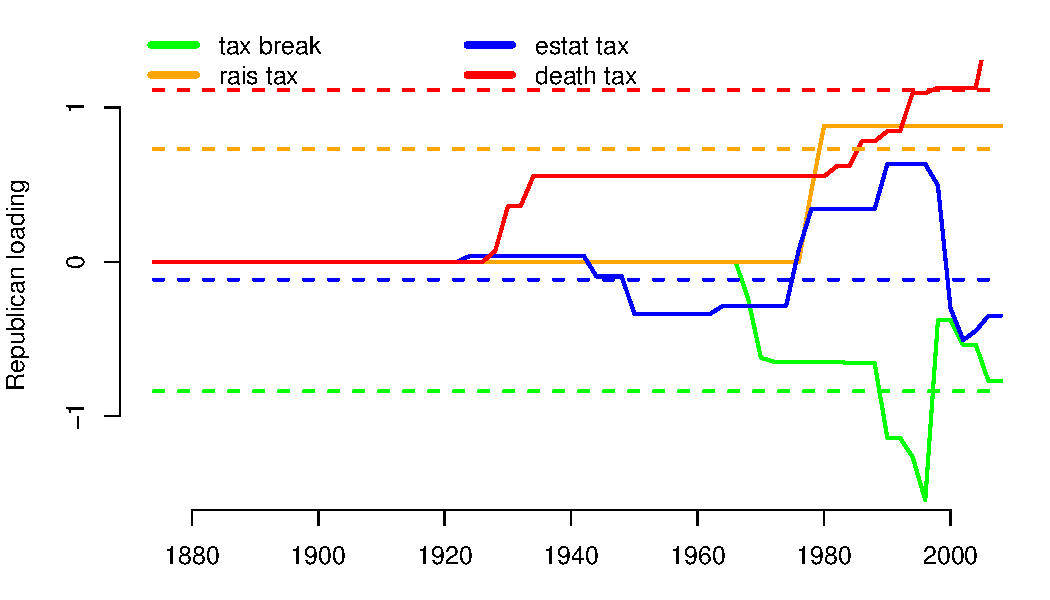
\includegraphics[width=\textwidth]{/home/taddy/project/politext/graphs/loaded_tax}

\vskip .5cm
The resulting fit has $\varphi_{tj}$ changing as a step function in $t$.

\end{frame}


\begin{frame}{Dynamic Phrase-Party Loadings: Race}

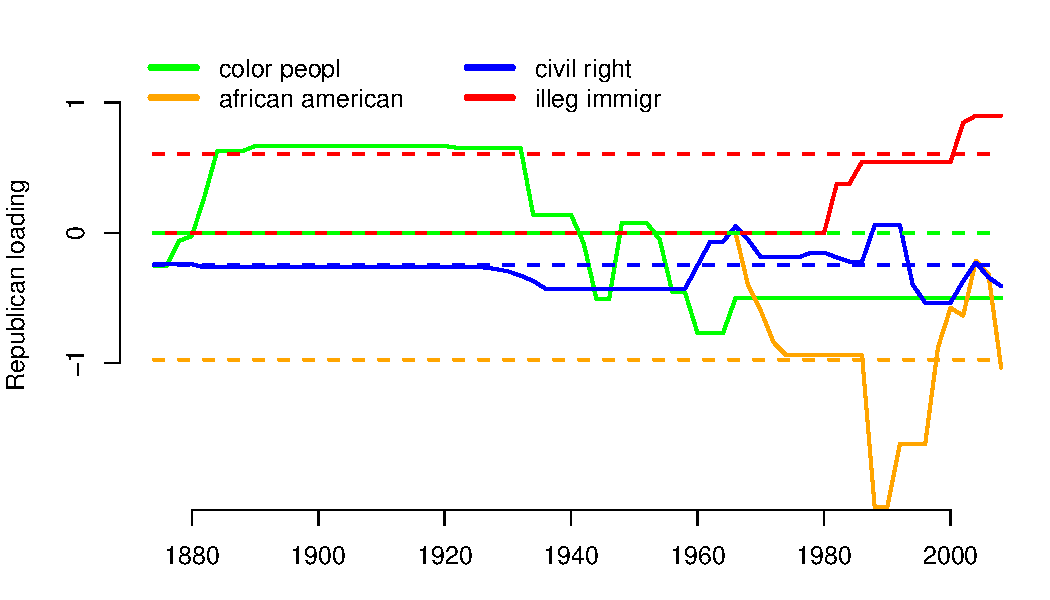
\includegraphics[width=\textwidth]{/home/taddy/project/politext/graphs/loaded_race}

\vskip .5cm
For this example, partisanship is robust to fixing $\varphi_{tj} = \varphi_{j}$.
\end{frame}

\begin{frame}{Polarization Results: Baseline Specification}


\includegraphics[width=\textwidth]{/home/taddy/project/politext/graphs/bic-polars_real_loglikelihood}

\vskip .5cm
We take $\bar z_{rt} = \frac{1}{n_{rt}} \sum_{i: r_i=r} z_{it}$ for
each party in each session, \\and the difference is our partisanship index.

\vskip .25cm
{\theme Partisanship of rhetoric has exploded since around 1980.}
\vskip -.25cm
\end{frame}

\begin{frame}{Nonparametric Bootstrap}


\includegraphics[width=\textwidth]{/home/taddy/project/politext/graphs/boot-bic-polars}

\vskip .5cm
1980 is also when real partisanship becomes more than \\$2SE$ away from that for random permutations.

\end{frame}

\begin{frame}{Penalization is a necessary ingredient}


\includegraphics[width=\textwidth]{/home/taddy/project/politext/graphs/noc-polars}


\vskip .5cm
These are the results corresponding to the end of each lasso path (most complex model)
\end{frame}

\begin{frame}{Robustness}


\includegraphics[width=\textwidth]{/home/taddy/project/politext/graphs/bic-polars_all}

\vskip .5cm
With BIC penalty selection, the same shape holds under a variety of specifications.  {\color{black!50} But notice: the controls do make a  difference.}
\end{frame}

\begin{frame}{Another application: racial segregation on the internet}

ComScore browser histories on the websites used in Gentzkow \texttt{+} Shapiro (2011), making visit-counts a function of $r_{it}$ black/white.

\vskip .25cm
\includegraphics[width=\textwidth]{/home/taddy/project/politext/graphs/Comscore-polars}

\vskip .25cm

Segregation online is high, but has been dropping since 2004.

\vskip -.25cm

\end{frame}


\begin{frame}
{wrap up}

\vskip .5cm
{Big picture: \theme  Give regression a chance!}  

\vskip .1cm
Everything here -- random effects, synthetic controls, lasso variable selection, utility interpretations -- is common in regression.  

\vskip .5cm
{\nv For example, Segregation Econometrics:} \\
~~~We've written down a model for choices, \\~~~and defined segregation in terms of that model.

\vskip .5cm
We can specify time dynamics and covariates inside this model.

\vskip .5cm
The same techniques that allow machine learners to avoid overfit in prediction can be used to recover representative model fits.


\begin{center}
\huge
Thanks!
\end{center}

\end{frame}

\end{document}
























